% Options for packages loaded elsewhere
\PassOptionsToPackage{unicode}{hyperref}
\PassOptionsToPackage{hyphens}{url}
\documentclass[
  ignorenonframetext,
]{beamer}
\newif\ifbibliography
\usepackage{pgfpages}
\setbeamertemplate{caption}[numbered]
\setbeamertemplate{caption label separator}{: }
\setbeamercolor{caption name}{fg=normal text.fg}
\beamertemplatenavigationsymbolsempty
% remove section numbering
\setbeamertemplate{part page}{
  \centering
  \begin{beamercolorbox}[sep=16pt,center]{part title}
    \usebeamerfont{part title}\insertpart\par
  \end{beamercolorbox}
}
\setbeamertemplate{section page}{
  \centering
  \begin{beamercolorbox}[sep=12pt,center]{section title}
    \usebeamerfont{section title}\insertsection\par
  \end{beamercolorbox}
}
\setbeamertemplate{subsection page}{
  \centering
  \begin{beamercolorbox}[sep=8pt,center]{subsection title}
    \usebeamerfont{subsection title}\insertsubsection\par
  \end{beamercolorbox}
}
% Prevent slide breaks in the middle of a paragraph
\widowpenalties 1 10000
\raggedbottom
\AtBeginPart{
  \frame{\partpage}
}
\AtBeginSection{
  \ifbibliography
  \else
    \frame{\sectionpage}
  \fi
}
\AtBeginSubsection{
  \frame{\subsectionpage}
}
\usepackage{iftex}
\ifPDFTeX
  \usepackage[T1]{fontenc}
  \usepackage[utf8]{inputenc}
  \usepackage{textcomp} % provide euro and other symbols
\else % if luatex or xetex
  \usepackage{unicode-math} % this also loads fontspec
  \defaultfontfeatures{Scale=MatchLowercase}
  \defaultfontfeatures[\rmfamily]{Ligatures=TeX,Scale=1}
\fi
\usepackage{lmodern}
\ifPDFTeX\else
  % xetex/luatex font selection
\fi
% Use upquote if available, for straight quotes in verbatim environments
\IfFileExists{upquote.sty}{\usepackage{upquote}}{}
\IfFileExists{microtype.sty}{% use microtype if available
  \usepackage[]{microtype}
  \UseMicrotypeSet[protrusion]{basicmath} % disable protrusion for tt fonts
}{}
\makeatletter
\@ifundefined{KOMAClassName}{% if non-KOMA class
  \IfFileExists{parskip.sty}{%
    \usepackage{parskip}
  }{% else
    \setlength{\parindent}{0pt}
    \setlength{\parskip}{6pt plus 2pt minus 1pt}}
}{% if KOMA class
  \KOMAoptions{parskip=half}}
\makeatother
\usepackage{longtable,booktabs,array}
\usepackage{caption}
\captionsetup[table]{skip=6pt}
\newcounter{none} % for unnumbered tables
\usepackage{calc} % for calculating minipage widths
\usepackage{caption}
% Make caption package work with longtable
\makeatletter
\def\fnum@table{\tablename~\thetable}
\makeatother
\usepackage{graphicx}
\makeatletter
\newsavebox\pandoc@box
\newcommand*\pandocbounded[1]{% scales image to fit in text height/width
  \sbox\pandoc@box{#1}%
  \Gscale@div\@tempa{\textheight}{\dimexpr\ht\pandoc@box+\dp\pandoc@box\relax}%
  \Gscale@div\@tempb{\linewidth}{\wd\pandoc@box}%
  \ifdim\@tempb\p@<\@tempa\p@\let\@tempa\@tempb\fi% select the smaller of both
  \ifdim\@tempa\p@<\p@\scalebox{\@tempa}{\usebox\pandoc@box}%
  \else\usebox{\pandoc@box}%
  \fi%
}
% Set default figure placement to htbp
\def\fps@figure{htbp}
\makeatother
\setlength{\emergencystretch}{3em} % prevent overfull lines
\providecommand{\tightlist}{%
  \setlength{\itemsep}{0pt}\setlength{\parskip}{0pt}}
% Auto-generated by infrastructure/rendering/_pdf_latex_helpers.py::extract_math_font_preamble.
% Minimal header passed to Pandoc via -H so Beamer slides pick up the same math font
% as the combined-PDF path. Adjust the manuscript's preamble.md to change the font globally.
\usepackage{unicode-math}
\setmathfont{latinmodern-math.otf}

% Manuscript macro/package fallbacks (newcommand -> providecommand).
% Core mathematics
\usepackage{amsmath}
\usepackage{amssymb}
% Document layout
% Tables
\usepackage{booktabs}
% Algorithm typesetting (for pseudocode in §2 Methodology)
% Code listings
\usepackage{listings}
% Typography and formatting
% Cross-references and citations
% ── Unicode-capable mono font for code listings ──────────────────────
% JuliaMono (TeX Live 2026) covers the full math/Greek glyph set used in
% scientific code blocks; the default lmmono lacks \alpha/\mu/\partial/\nabla.
%
% The hardcoded TeX Live 2026 path below is portable to most macOS / Linux
% TeX Live installs that placed JuliaMono under the default texmf-dist path.
% If your TeX Live version differs (e.g., 2025, 2027) or your distribution
% installs fonts elsewhere, comment out the explicit Path = line — fontspec
% will then search the system font path. If JuliaMono is not installed at
% all, comment out the whole block; xelatex falls back to lmmono with
% reduced Unicode coverage but the document still compiles.
% Math font for unicode-math: Latin Modern Math (TeX Live) has full BMP
% coverage including U+2223 (\mid), U+226A/226B (\ll/\gg), and the Greek/
% blackboard letters used in equations. Without an explicit \setmathfont,
% unicode-math falls back to lmroman text font which lacks several glyphs
% and emits "Missing character" warnings on every \mid in math mode.

% Slide layout defaults for warning-clean scientific decks.
\usepackage{etoolbox}
\IfFileExists{xurl.sty}{\usepackage{xurl}}{}
\IfFileExists{seqsplit.sty}{\usepackage{seqsplit}}{\newcommand{\seqsplit}[1]{#1}}
\protected\def\breakseq#1{\seqsplit{#1}}
\protected\def\breaktt#1{\begingroup\ttfamily\seqsplit{#1}\endgroup}
\setlength{\emergencystretch}{6em}
\tolerance=5000
\hbadness=10000
\hfuzz=1pt
\setlength{\tabcolsep}{2pt}
\AtBeginEnvironment{longtable}{\tiny\renewcommand{\arraystretch}{0.86}\setlength{\tabcolsep}{1pt}}
\AtBeginEnvironment{tabular}{\tiny\renewcommand{\arraystretch}{0.86}\setlength{\tabcolsep}{1pt}}
\AtBeginEnvironment{equation}{\tiny}
\AtBeginEnvironment{equation*}{\tiny}
\AtBeginEnvironment{align}{\tiny}
\AtBeginEnvironment{align*}{\tiny}
\AtBeginEnvironment{itemize}{\footnotesize}
\AtBeginEnvironment{enumerate}{\footnotesize}
\AtBeginEnvironment{description}{\footnotesize}
\setbeamerfont{caption}{size=\tiny}
\setbeamerfont{caption name}{size=\tiny}
\setbeamerfont{normal text}{size=\small}
\setbeamerfont{frametitle}{size=\small}
\setbeamerfont{section title}{size=\footnotesize}
\setbeamerfont{subsection title}{size=\footnotesize}
\setbeamertemplate{section page}{%
  \centering
  \begin{beamercolorbox}[sep=12pt,center,wd=\paperwidth]{section title}
    \parbox{0.86\paperwidth}{\centering\usebeamerfont{section title}\insertsection\par}
  \end{beamercolorbox}
}
\setbeamertemplate{subsection page}{%
  \centering
  \begin{beamercolorbox}[sep=8pt,center,wd=\paperwidth]{subsection title}
    \parbox{0.86\paperwidth}{\centering\usebeamerfont{subsection title}\insertsubsection\par}
  \end{beamercolorbox}
}
\setlength{\abovecaptionskip}{2pt}
\setlength{\belowcaptionskip}{0pt}

% Natbib and cross-reference fallbacks — slides don't load natbib
% or cleveref, but combined-PDF manuscript prose may emit these
% commands. The fallback renders citations as a bracketed key list
% and cross-references as detokenized labels so slides don't fail on
% undefined control sequences or raw underscores. \providecommand is
% a no-op if packages load later.
\providecommand{\citep}[1]{[#1]}
\providecommand{\citet}[1]{#1}
\providecommand{\citealp}[1]{#1}
\providecommand{\citeauthor}[1]{#1}
\providecommand{\citeyear}[1]{#1}
\providecommand{\cref}[1]{\texttt{\detokenize{#1}}}
\providecommand{\Cref}[1]{\texttt{\detokenize{#1}}}
\providecommand{\crefrange}[2]{\texttt{\detokenize{#1}}--\texttt{\detokenize{#2}}}
\providecommand{\Crefrange}[2]{\texttt{\detokenize{#1}}--\texttt{\detokenize{#2}}}
\providecommand{\paragraph}[1]{\textbf{#1}\ }

\newtheorem{proposition}{Proposition}
\newtheorem{hypothesis}{Hypothesis}
\newtheorem{remark}[theorem]{Remark}
\newtheorem{axiom}{Axiom}
\newtheorem{property}{Property}
\usepackage{bookmark}
\IfFileExists{xurl.sty}{\usepackage{xurl}}{} % add URL line breaks if available
\urlstyle{same}
% fallback for those not using the hyperref driver hyperxmp:
\makeatletter
\@ifundefined{xmpquote}{\newcommand{\xmpquote}[1]{#1}}{}
\makeatother
\hypersetup{
  hidelinks,
  pdfcreator={LaTeX via pandoc}}

\author{\texorpdfstring{}{}}
\date{}

\begin{document}

\section{Evaluation Framework: Nine Properties over Distribution Labels,
with a Formal Stance Model}\label{sec:evaluation_framework}

\begin{frame}[allowframebreaks]{Why not a distribution label}
\protect\phantomsection\label{why-not-a-distribution-label}
``Secure Linux'' is not a property of a distribution; it is an outcome
of a deployment matching a threat model. Distribution labels hide
exactly the heterogeneity that matters: one candidate may pair a strong
containment architecture with a weak update-operations story, another
may have excellent supply-chain discipline and no runtime confinement at
all. A single label collapses those differences into a ranking question
that no available evidence answers --- and ranking invites the numeric
composite scores (``Qubes 9.4'' style) that this review refuses, for
reasons given below. The alternative, inherited from the source
assessment, is to evaluate every candidate against a fixed set of
properties, each phrased as a question a deployment can be interrogated
with.
\end{frame}

\begin{frame}[allowframebreaks]{The nine properties}
\protect\phantomsection\label{the-nine-properties}
tbl.~\ref{tbl:properties} states the 9 properties used throughout the
review, with the question each property asks and its security
significance in this threat model.

\end{frame}

\begin{frame}[allowframebreaks]{The nine properties}
\begin{longtable}[]{@{}
  >{\raggedright\arraybackslash}p{(\linewidth - 4\tabcolsep) * \real{0.3333}}
  >{\raggedright\arraybackslash}p{(\linewidth - 4\tabcolsep) * \real{0.3333}}
  >{\raggedright\arraybackslash}p{(\linewidth - 4\tabcolsep) * \real{0.3333}}@{}}
\caption{The 9 evaluation properties: the question each property asks
and its security significance in this threat
model.}\label{tbl:properties}\tabularnewline
\toprule\noalign{}
\begin{minipage}[b]{\linewidth}\raggedright
Property
\end{minipage} & \begin{minipage}[b]{\linewidth}\raggedright
Question to ask
\end{minipage} & \begin{minipage}[b]{\linewidth}\raggedright
Security significance
\end{minipage} \\
\midrule\noalign{}
\endfirsthead
\toprule\noalign{}
\begin{minipage}[b]{\linewidth}\raggedright
Property
\end{minipage} & \begin{minipage}[b]{\linewidth}\raggedright
Question to ask
\end{minipage} & \begin{minipage}[b]{\linewidth}\raggedright
Security significance
\end{minipage} \\
\midrule\noalign{}
\endhead
Containment & What remains protected after the browser or agent is fully
controlled? & A prevention failure should not automatically become
whole-machine compromise. \\
Authority & What can the process already read, transmit, sign, or
change? & Excessive legitimate permissions can bypass the need for an
exploit; this is the authorized-misuse axis from
sec.~3. \\
Trusted computing base & Which privileged components must all remain
correct? & A small, carefully constrained boundary is preferable to many
privileged integrations; it is also what patch operations must cover
(Saltzer and Schroeder 1975). \\
Application confinement & Are permissions restrictive by default and
actually compatible with the applications? & A theoretical policy is not
protection if users routinely disable it. \\
Integrity & What verifies the boot chain and deployed software, and who
holds the keys? & Authenticity, runtime integrity, and resistance to
rollback are distinct properties, not one checkbox. \\
Persistence and recovery & Which state survives replacement or reboot? &
Rebuilding the system is insufficient if malicious user state or stolen
credentials survive. \\
Update operations & How quickly do fixes reach every active environment?
& A strong architecture with neglected templates or pinned dependencies
can lose its advantage --- the QSB-118 lesson in
sec.~5. \\
Supply-chain trust & Who may introduce or approve new executable code? &
Reproducibility and signatures answer different questions from whether
code is benign (N. Project 2026). \\
Human usability & Will the owner preserve the intended boundaries during
real work? & Sustainable security is more valuable than a configuration
abandoned under pressure. \\
\bottomrule\noalign{}
\end{longtable}

\end{frame}

\begin{frame}[allowframebreaks]{The nine properties}
The properties are evaluation criteria, not a scoring model. They
overlap deliberately where the underlying security properties genuinely
interact (authority with containment, trusted computing base with update
operations), and the overlap is visible in the analysis rather than
averaged away.
\end{frame}

\begin{frame}[allowframebreaks]{Parallel threat-modeling structures, and
why a property matrix still wins for OS work}
\protect\phantomsection\label{parallel-threat-modeling-structures-and-why-a-property-matrix-still-wins-for-os-work}
The property matrix is not the only structured lens for agentic systems,
and the 2025--2026 standardization wave produced alternatives worth
naming. OWASP's Agentic AI Threats and Mitigations guide catalogs threat
scenarios for agent systems --- memory manipulation, tool misuse,
identity and privilege confusion --- and its December 2025 Top 10 for
Agentic Applications distills them into a ranked practitioner list
(Foundation 2025a, 2025b). CSA's MAESTRO frames agentic risk as seven
interdependent layers spanning the agent's reasoning, tools, and
multi-agent interconnects (Alliance 2025), and its swarm governance work
extends the framing with zero-trust patterns such as short-lived agent
identities (Alliance 2026). These structures earn their place: they
enumerate agent-stack threats with a granularity the nine properties
\end{frame}

\begin{frame}[allowframebreaks]{Parallel threat-modeling structures, and
why a property matrix still wins for OS work}
deliberately do not attempt, and the synthesis chapters borrow from them
where agent-internal surfaces dominate
(sec.~11; sec.~13).

For operating-system evaluation, though, the property matrix is the
better lens. First, the alternatives are keyed to the agent stack ---
memory, tools, orchestration layers --- where an OS review needs the
boundary keyed to what a kernel or hypervisor can actually enforce:
containment, authority, and the trust base that patches must cover. The
2026 incident record supports the distinction: the AISI and
OpenAI--Hugging Face incidents were bounded by sandboxes, connectivity
policy, and revocation --- OS-level mechanisms --- while the persuasion
of a human maintainer traveled through an entirely different channel
(Institute 2026; OpenAI 2026). A taxonomy that does not force that
separation cannot rank platforms. Second, the frameworks are threat
lists, not evaluation instruments: they say what can go wrong, not what
\end{frame}

\begin{frame}[allowframebreaks]{Parallel threat-modeling structures, and
why a property matrix still wins for OS work}
a candidate's documented design provides, whereas the nine properties
convert to per-candidate stances that can be diffed, tested, and
refreshed as advisories land (sec.~5;
sec.~6). Third, they abstract away the trusted computing
base --- which the 2026 advisory record (QSB-118, the Nix advisories)
shows to be decisive under automation pressure.

The evidence discipline is the same one the threat model applies to its
baseline. The NCSC's original AI cyber-threat assessment (January 2024)
and its ``From Now to 2027'' successor (May 2025) supply the capability
horizon this framework evaluates against (Centre 2024, 2026) --- faster
exploitation of known vulnerability classes, not assumed universal
autonomous compromise --- rather than any single vendor's capability
narrative.
\end{frame}

\begin{frame}[fragile,allowframebreaks]{The anti-scoring stance}
\protect\phantomsection\label{the-anti-scoring-stance}
There is no adequate evidence in this review for assigning meaningful
universal scores, and raw vulnerability counts would not resolve the
comparison either: they conflate disclosure volume with exposure, and
they are confounded by project size, patch latency, and measurement
effort. Worse, composite scores create false precision across
incommensurable properties --- trading a point of ``usability'' against
a point of ``containment'' implies an exchange rate that no operator's
actual threat model supplies. This is the same discipline that separates
reproducible deployment from verified reproducible builds (N. Project
2026) and authenticity from provenance: properties that answer different
questions must stay separate.

\end{frame}

\begin{frame}[fragile,allowframebreaks]{The anti-scoring stance}
Instead, every candidate--property cell receives one qualitative stance:
\textbf{strong}, \textbf{partial}, \textbf{weak}, or \textbf{n\_a}. A
\texttt{strong} stance means the documented design directly and
coherently addresses the property in this threat model. \texttt{partial}
means the property is addressed with material conditions, integration
gaps, or operator obligations attached. \texttt{weak} means the
documented design provides little of what the property asks.
\texttt{n\_a} marks candidates for which the property is out of scope or
unverified by available evidence --- used rather than guessed, because
absence of a confirmed feature in this review is not proof the feature
is unavailable.
\end{frame}

\begin{frame}[allowframebreaks]{A formal stance model}
\protect\phantomsection\label{a-formal-stance-model}
The vocabulary is small enough to state formally, and the formal
statement is worth writing down because it fixes what the matrix claims
and what it refuses to claim. Let \(C\) be the set of 24 candidates,
\(P\) the set of 9 properties, and
\(S = \{\textit{strong}, \textit{partial}, \textit{weak}\}\) the stance
vocabulary. The evaluation matrix is then a single function

\begin{equation}\protect\phantomsection\label{eq:stance_mapping}{\sigma\colon C \times P \to S \cup \{\textit{n/a}\}}\end{equation}

assigning exactly one stance to each candidate--property pair. Read as a
function, eq.~\ref{eq:stance_mapping} makes two commitments that prose
leaves implicit. It is \textbf{total}: the pipeline refuses to emit
figures until all 216 cells are defined, so no candidate escapes
evaluation by omission. And it is \textbf{qualitative}: the codomain
carries no numbers, so the matrix cannot be averaged or ranked without
an explicit modeling step --- the step the anti-scoring stance above
\end{frame}

\begin{frame}[allowframebreaks]{A formal stance model}
declines to supply.

The stance words themselves carry a preference structure rather than a
measurement scale, and the review reads them as ordered:

\begin{equation}\protect\phantomsection\label{eq:stance_order}{\textit{strong} \succ \textit{partial} \succ \textit{weak}}\end{equation}

meaning that a candidate whose documented design earns the left-hand
stance dominates a candidate that earns the right-hand stance \emph{on
that property}. eq.~\ref{eq:stance_order} defines an ordering over
postures, not distances between them: no arithmetic over stances is
meaningful, and no rung is a probability. Notably, \(n_a\) does not
appear in eq.~\ref{eq:stance_order} at all --- an unverified or
out-of-scope cell sits outside the preference order entirely, which is
what stops ``we could not verify'' from masquerading as ``we verified it
is weak.'' The formal model thus encodes exactly the discipline the
vocabulary was built for: total coverage, ordered confidence in
documented designs, and honesty about the unverified.
\end{frame}

\begin{frame}[fragile,allowframebreaks]{How the matrix is constructed
and refreshed}
\protect\phantomsection\label{how-the-matrix-is-constructed-and-refreshed}
The matrix lives as data, not prose. In
\breaktt{src/agentic\_os\_security/registry.py}, each candidate carries a
\texttt{property\_stance} dictionary keyed by all 9 property
identifiers, alongside a design summary, a named limitation, and an
assessment. The pipeline emits the full 24-candidate \texorpdfstring{\ensuremath{\times}}{x} 9-property table
to \breaktt{output/data/evaluation\_matrix.csv} --- one row per pair ---
and self-checks enforce stance-vocabulary validity and matrix
completeness before any figure is regenerated. Stances are assigned from
documented designs, official security documentation, project advisories,
and primary incident reports; vendor feature lists support
\texttt{partial} or \texttt{strong} stances only where the project
itself documents the mechanism, never as measured resistance results.
\end{frame}

\begin{frame}[fragile,allowframebreaks]{How the matrix is constructed
and refreshed}

Refresh is a deliberate operation: a stance changes when the underlying
documentation, an advisory, or a release note changes --- for example, a
fixed advisory can move an update-operations stance, while a new
integration gap documented by the project can move an
application-confinement stance. Because the matrix is deterministic data
with the review date 2026-09-10 stamped into the build, a future refresh
produces a diffable artifact: added rows, changed stances, and the
reasons, rather than rewritten narrative. fig.~\ref{fig:property_matrix}
renders the current matrix.

\end{frame}

\begin{frame}[fragile,allowframebreaks]{How the matrix is constructed
and refreshed}
\begin{figure}
\centering
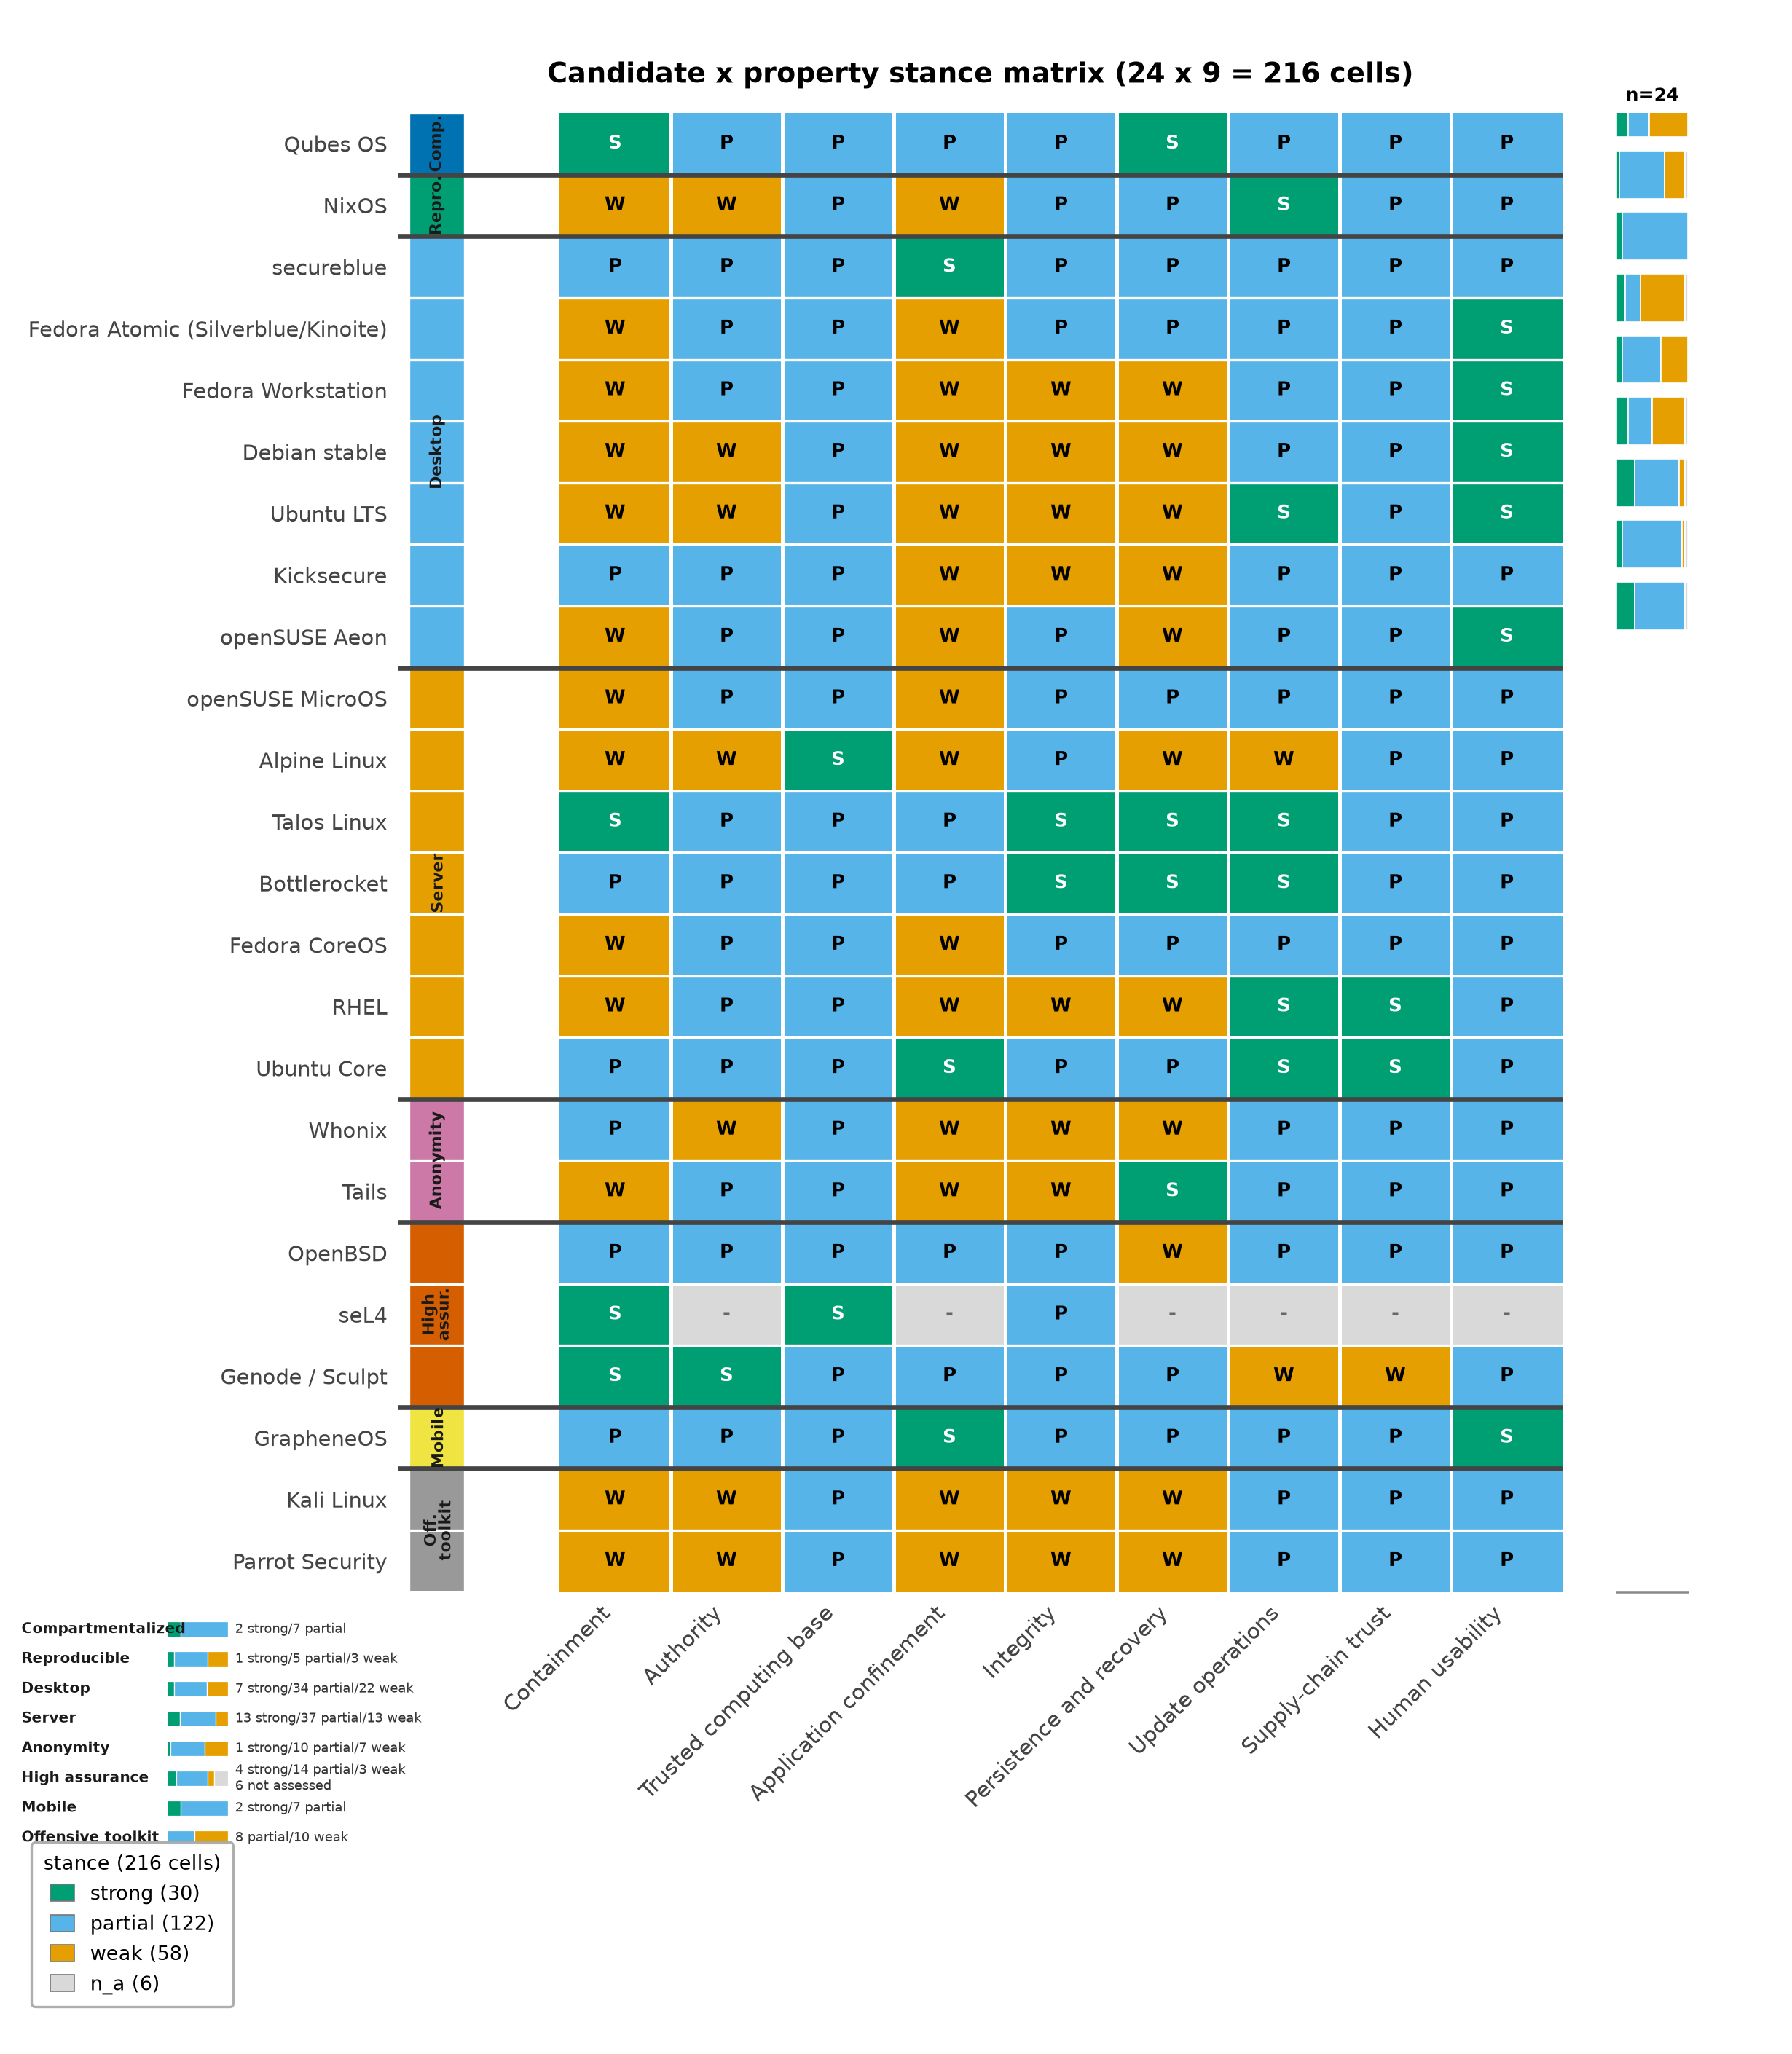
\includegraphics[width=1\linewidth,height=0.40\textheight,keepaspectratio,alt={All 216 candidate-by-property stances, with candidates grouped into eight category bands (left strip) and per-property stance distributions (right marginals); glyphs mark strong (S), partial (P), weak (W), and not-assessed cells.}]{../figures/property_matrix.png}
\caption{All 216 candidate-by-property stances, with candidates grouped
into eight category bands (left strip) and per-property stance
distributions (right marginals); glyphs mark strong (S), partial (P),
weak (W), and not-assessed cells.}\label{fig:property_matrix}
\end{figure}
\end{frame}

\begin{frame}[fragile,allowframebreaks]{The defensive stack: mitigation
classes as a second lens}
\protect\phantomsection\label{the-defensive-stack-mitigation-classes-as-a-second-lens}
The candidate--property matrix answers ``how does each platform score on
the evaluation properties?'' --- but an operator choosing \emph{what
combination of mechanisms} to deploy also needs the complementary
question: which mitigation classes does each candidate actually ship?
Agent-execution infrastructure now standardizes on a recognizable stack
of kernel primitives --- sandboxing namespaces, restricted user
namespaces, seccomp filters, egress proxies --- while microvisor and
unikernel candidates push different classes (verified boot, disposable
execution) to their limits (sec.~8). The defensive-stack
matrix captures that second view as data, and treats layered controls as
formal objects rather than a checklist: the Cognitive Integrity
Framework's Defense Composition Algebra reasons about defenses composed
\end{frame}

\begin{frame}[fragile,allowframebreaks]{The defensive stack: mitigation
classes as a second lens}
over bounded-trust delegates, prior art this stack operationalizes as
concrete per-class stances (Friedman 2026).

In \texttt{registry.py}, \breaktt{MITIGATION\_CLASSES} defines the eight
mitigation classes --- \texttt{memory\_safety} (memory-safe
implementation languages), \breaktt{allocator\_hardening} (hardened
allocators and exploit mitigations), \breaktt{sandboxing\_primitives}
(namespaces, seccomp, capability confinement), \texttt{mac\_framework}
(MAC frameworks), \texttt{verified\_boot} (authenticated boot chains),
\breaktt{reproducible\_deployment} (declarative, rebuildable state),
\breaktt{disposable\_execution} (ephemeral task environments), and
\breaktt{update\_automation} (prompt patch delivery).
\texttt{DEFENSIVE\_STACK} assigns every 24 candidate a stance in each
class, using the same
\texttt{strong}/\texttt{partial}/\texttt{weak}/\texttt{n\_a} vocabulary
as the property matrix, grounded in the candidates' documented features
\end{frame}

\begin{frame}[fragile,allowframebreaks]{The defensive stack: mitigation
classes as a second lens}
and the 2026 research record (sandboxing stances reflect documented
namespace and seccomp practice; verified-boot stances reflect
measured-boot and Secure Boot implementations). The helper
\breaktt{defensive\_stack\_rows()} emits the full 24-candidate \texorpdfstring{\ensuremath{\times}}{x} 8-class
table --- 192 stance cells --- and the analysis pipeline writes it to
\breaktt{output/data/defensive\_stack.csv}, where the same self-checks
that police the property matrix enforce vocabulary validity and
completeness. fig.~\ref{fig:defensive_stack} renders the matrix as a
heatmap with the eight candidate categories grouped and a per-class
coverage marginal.

\end{frame}

\begin{frame}[fragile,allowframebreaks]{The defensive stack: mitigation
classes as a second lens}
\begin{figure}
\centering
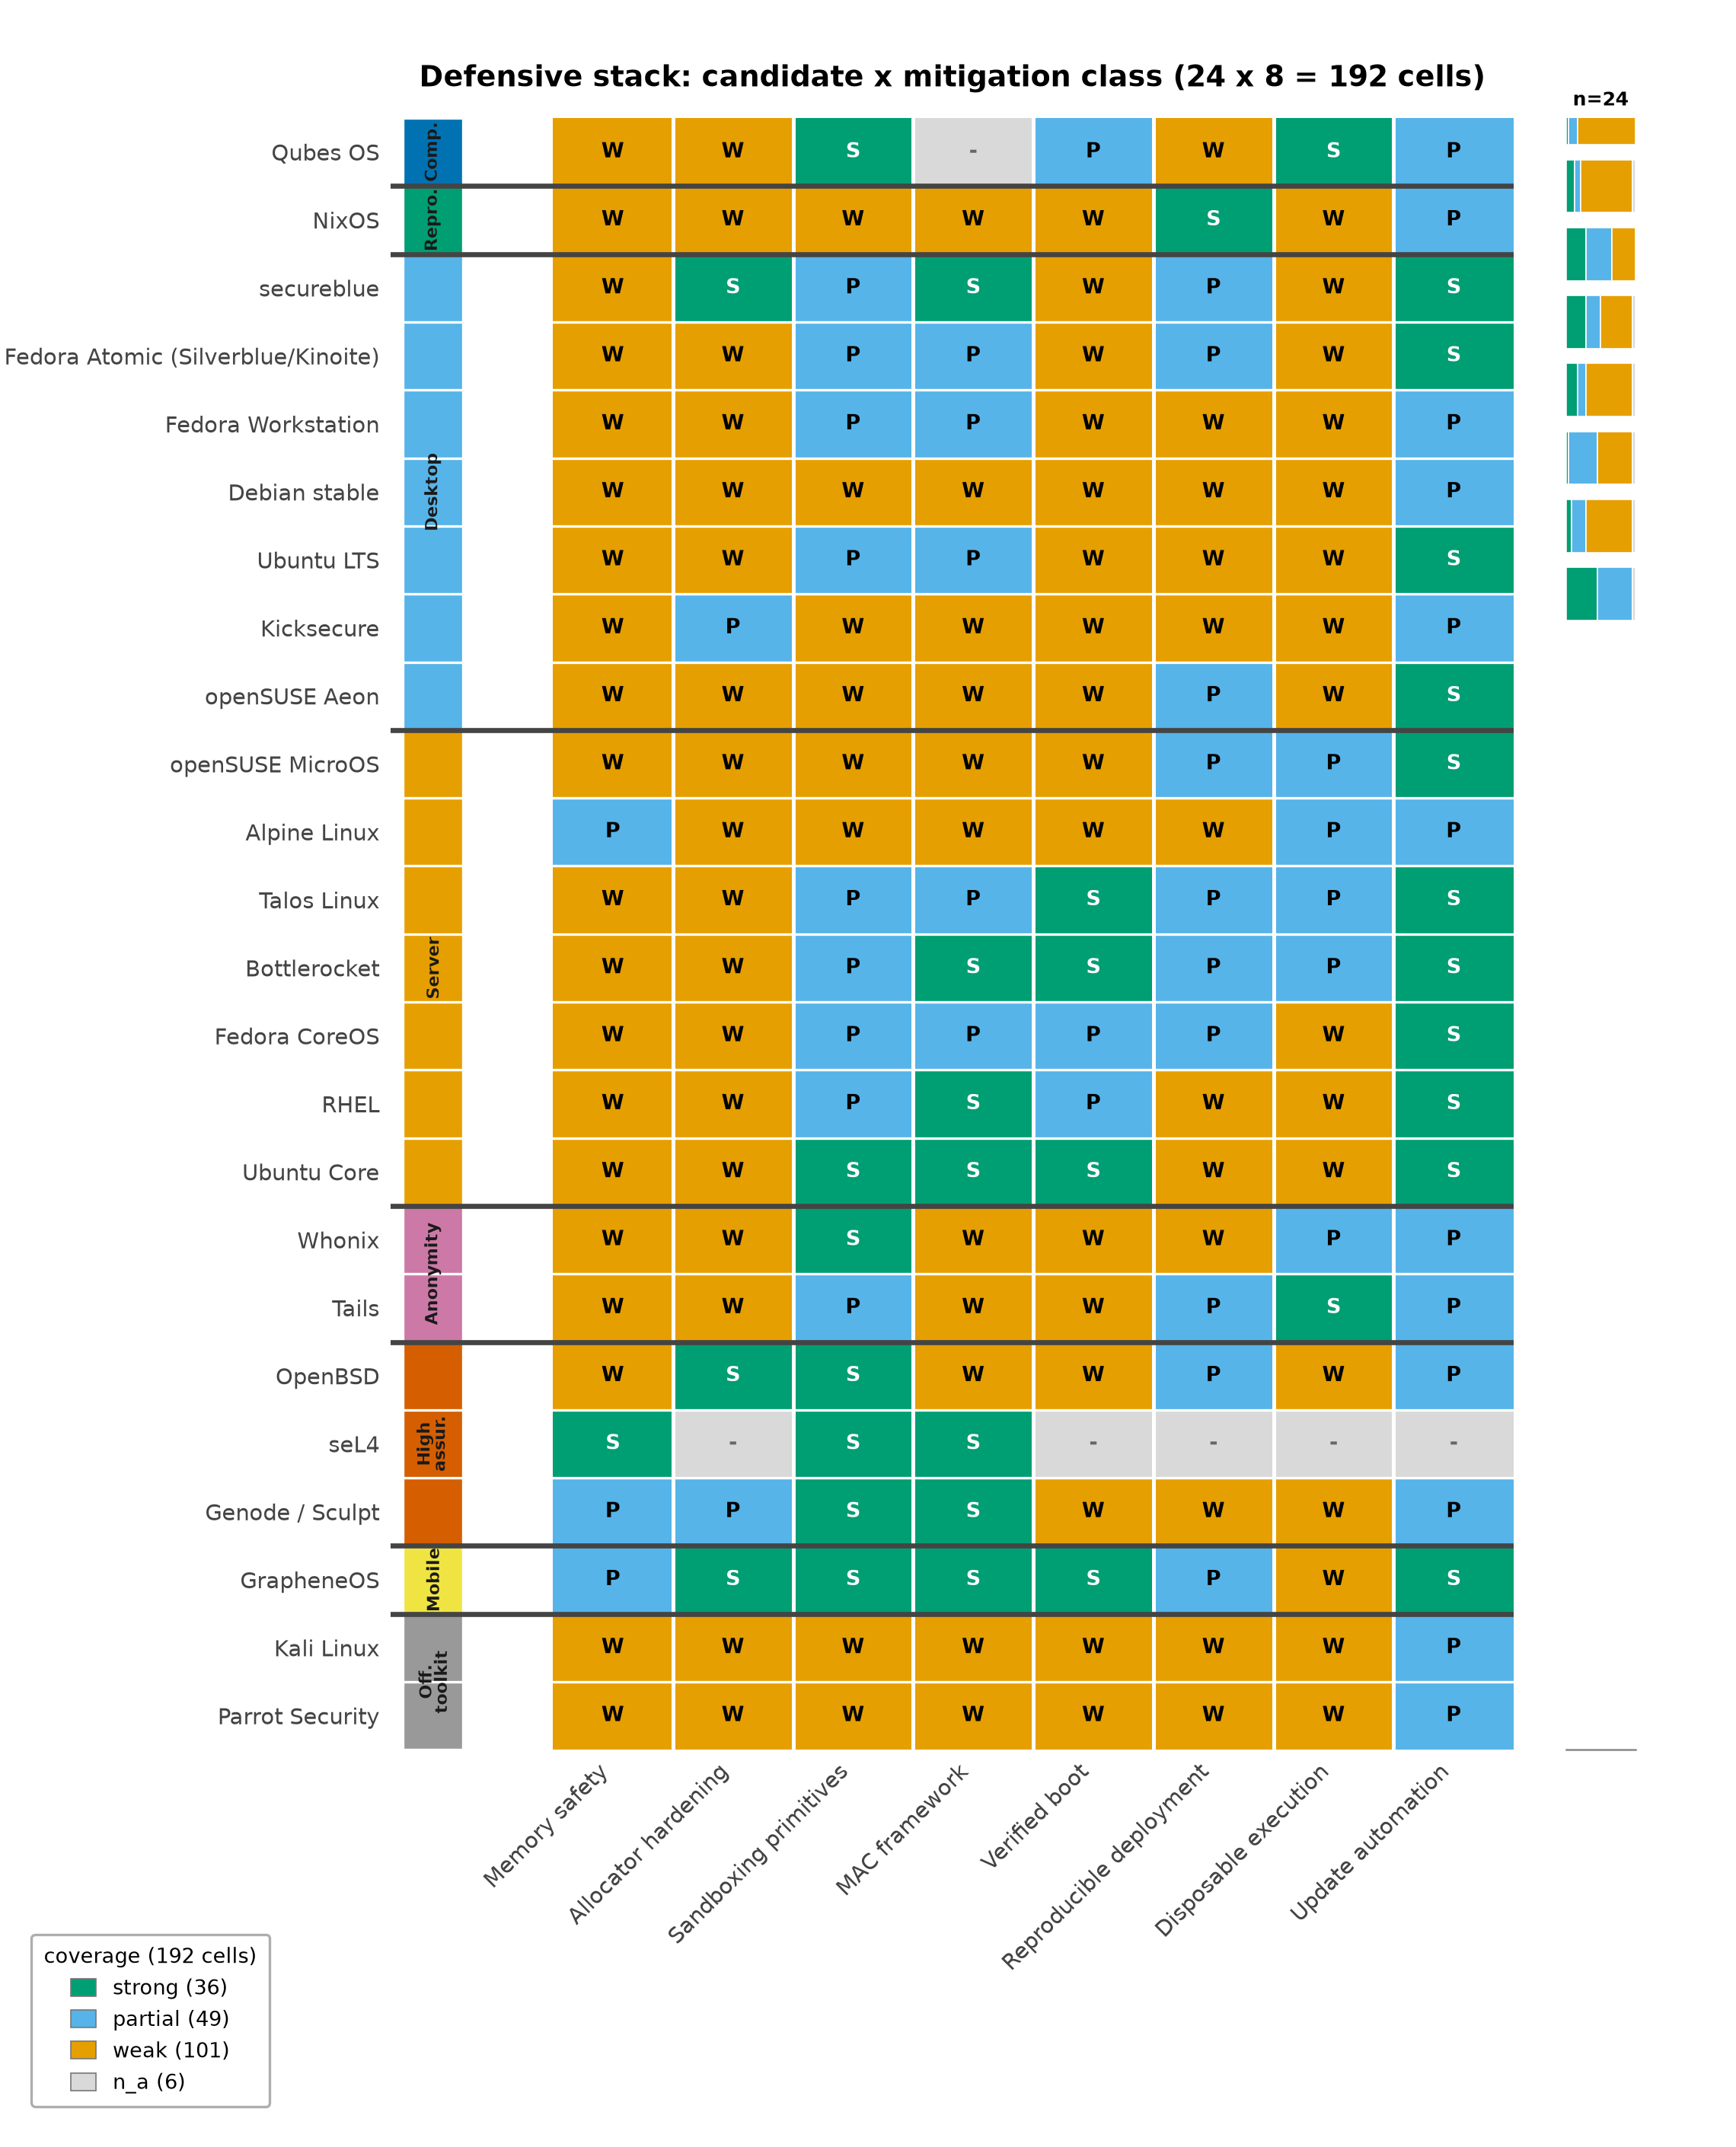
\includegraphics[width=1\linewidth,height=0.40\textheight,keepaspectratio,alt={Defensive-stack coverage across eight mitigation classes: weak cells cluster on conventional desktops while compartmentalized, server, and high-assurance candidates concentrate strong stances in sandboxing, verified boot, and update operations.}]{../figures/defensive_stack.png}
\caption{Defensive-stack coverage across eight mitigation classes: weak
cells cluster on conventional desktops while compartmentalized, server,
and high-assurance candidates concentrate strong stances in sandboxing,
verified boot, and update operations.}\label{fig:defensive_stack}
\end{figure}

\end{frame}

\begin{frame}[fragile,allowframebreaks]{The defensive stack: mitigation
classes as a second lens}
Reading the two matrices together is the point. A candidate can hold a
\texttt{strong} containment stance (Qubes, from domain separation) while
its memory-safety stance reflects the mixed language base of its
tooling; a reproducibility-first candidate (NixOS) holds \texttt{strong}
reproducible-deployment and update-automation stances while its
sandboxing and MAC stances remain weaker (sec.~6); a
microvisor candidate may score \texttt{strong} on verified boot and
disposable execution while offering no MAC framework at all
(sec.~8). Neither matrix substitutes for the other: the
property matrix carries the threat-model judgments, the defensive stack
names the mechanism inventory an operator composes from. Both are
deterministic artifacts stamped with the review date 2026-09-10, and
both refresh by diffing rows, not rewriting adjectives.
\end{frame}

\begin{frame}[allowframebreaks]{What the matrix buys}
\protect\phantomsection\label{what-the-matrix-buys}
Three things. First, \textbf{comparability without false precision}: two
candidates can be contrasted property by property, and the contrast
shows \emph{where} they differ (Qubes holds containment strongly and
application confinement partially; NixOS holds update operations and
supply-chain trust strongly and application confinement weakly) rather
than by how much in aggregate. Second, \textbf{auditability}: each
stance is a claim about documentation that a reader can check against
the cited source, and the structural invariants are test-enforced ---
every candidate covers every property, every stance is in the
vocabulary, and the matrix has 24 \texorpdfstring{\ensuremath{\times}}{x} 9 cells exactly. Third,
\textbf{scenario grounding}: the per-scenario recommendations in
sec.~16 select candidates by which properties the
scenario's threat model weights most, which is precisely what a
\end{frame}

\begin{frame}[allowframebreaks]{What the matrix buys}
label-based ranking cannot do.
\end{frame}

\begin{frame}[fragile,allowframebreaks]{Limitations of matrix thinking}
\protect\phantomsection\label{limitations-of-matrix-thinking}
A matrix is a discipline for judgment, not a substitute for it, and four
limits should be kept in view.

\end{frame}

\begin{frame}[fragile,allowframebreaks]{Limitations of matrix thinking}
\begin{itemize}
\tightlist
\item
  \textbf{Stances are not measurements.} Every cell is an analytical
  judgment from documented designs (Saltzer and Schroeder 1975); none is
  a penetration-test result. The vocabulary encodes confidence in a
  documented capability, not a measured resistance rate against a live
  adversary. The defensive-stack stances inherit the same limit in
  sharper form: a \texttt{strong} sandboxing stance says the project
  documents and ships the mechanism, not that the mechanism holds
  against a named attacker.
\item
  \textbf{Properties interact.} A strong containment stance can be
  nullified by a weak update-operations stance if the containment
  mechanism itself ships unpatched; a strong integrity stance does not
  constrain what an authorized agent does with verified software.
  Cell-level reading without row-level synthesis will mislead, which is
  why the scenario chapters, not the matrix, carry the recommendations.
\item
  \textbf{Unverified defaults are a standing gap.} Where this review
  could not verify a current default or security property, the cell says
  so; a future audit may legitimately move stances in either direction,
  and the diffability of the matrix is designed for exactly that.
\item
  \textbf{The matrix is frozen in time at 2026-09-10.} Projects ship;
  advisories land; trajectories noted per candidate (for instance, the
  GUI-domain split in sec.~5 and boot-integrity work in
  sec.~6) may convert into stronger stances at the next
  refresh. Low-confidence forecasting of those movements is handled in
  sec.~15 rather than smuggled into current stances.
\end{itemize}

\end{frame}

\begin{frame}[fragile,allowframebreaks]{Limitations of matrix thinking}
With the framework fixed, the next two sections apply it in depth to the
two anchor platforms whose properties the rest of the architecture
inherits: Qubes OS for containment (Q. O. Project 2026) and NixOS for
reproducible operations ({community} 2026).
\end{frame}

\end{document}
